\chapter*{Introduzione}
\addcontentsline{toc}{chapter}{Introduzione}
Il mondo odierno è ormai pervaso dall'Intelligenza Artificiale. Uno dei settori di maggior interesse per la
ricerca in questo ambito è indubbiamente quello delle cosidette \emph{Self Driving Car}, ovvero
le macchine a guida autonoma. 
\begin{figure}
  \centering
  \parbox{5cm}{
  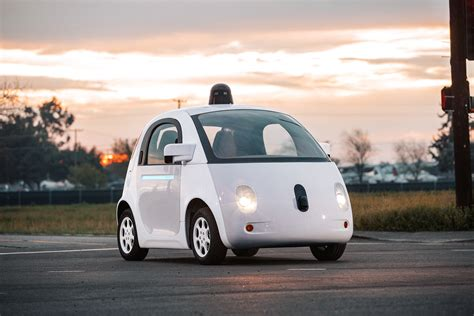
\includegraphics[width=5cm]{googlecar}
  \caption{self driving car di Google}
  \label{fig:google}}
  \qquad
  \begin{minipage}{5cm}
  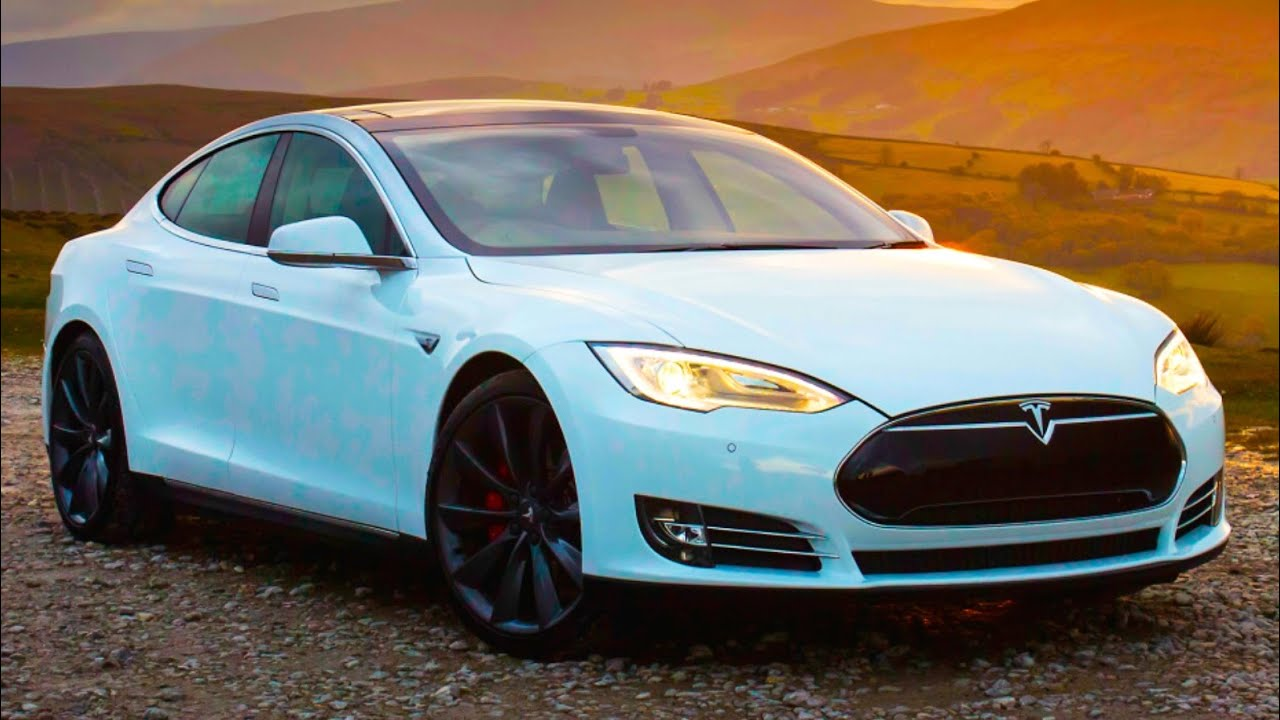
\includegraphics[width=5cm]{tesla}
  \caption{self driving car di Tesla}
  \label{fig:tesla}
  \end{minipage}
  \end{figure}
Grandi aziende quali \emph{Google} e \emph{Tesla} hanno già sviluppato
dei propri modelli(Figura \ref{fig:google} e \ref{fig:tesla}) e l'interesse per questo tipo di veicoli è sempre in  maggior crescita.
Per poter funzionare correttamente questi veicoli acquisiscono informazioni dall'ambiente circostante sotto forma di immagini.
Queste immagini vengono classificate da un sistema interno che, in base alle informazioni ricevute, decide l'azione da compiere(sterzare, accelerare, frenare ecc.).
Anni ed anni di sviluppo e ricerca hanno reso sempre più affidabili e sicuri  questi sistemi ma restano comunque presenti delle vulnerabilità. Una vulnerabilità
molto importante sono i cosiddetti \emph{Adversarial attacks}. Il meccanismo di questi attacchi è molto semplice:
\\
alle immagini raccolte dal sistema viene applicata una modifica impercettibile a occhio umano ma in grado di causare un errore di classificazione che può portare, ad esempio, una macchina ad accelerare quando
dovrebbe frenare. La ricerca su questi tipi di attacchi quindi è fondamentale per garantire l'affidabilità dei veicoli a guida autonoma.
Lo scopo di questa tesi è l'implementazione di \emph{Adversarial Attacks} contro modelli di guida autonoma in ambiente simulato.
Il lavoro è cosi suddiviso:
\begin{itemize}
  \item \textbf{Capitolo 1:} descrizione dei fondamenti teorici alla base dei sistemi di guida autonoma e più in generale dei sistemi intelligenti
  \item \textbf{Capitolo 2:} descrizione degli strumenti utilizzati: in particolare vengono presentati \emph{l'Adversarial Robustness Toolbox} e il simulatore \emph{Carla}
  \item \textbf{Capitolo 3:} descrizione degli attacchi scelti per l'implementazione e  motivazioni per le scelte effettuate
  \item \textbf{Capitolo 4:} Implementazione e risultati
  \item \textbf{Capitolo 5:} Conclusioni e possibili sviluppi futuri
  
\end{itemize}


